% Chapter 1

\chapter{Background Literature} % Main chapter title

\label{Chapter2} % For referencing the chapter elsewhere, use \ref{Chapter1} 

\lhead{Chapter 2. \emph{Background Knowledge}} % This is for the header on each page - perhaps a shortened title

%----------------------------------------------------------------------------------------

Historically, computer networks have always been relatively blackboxed entities that provide no substantial
facilities for configuration. The devices that are present in them, from traditional switches and routers, to other
middleware like firewalls and network address translators, often execute software that is proprietary, and hence
rigid by nature.
\newline
These devices are configured by network aaadministrators using highly specialised interfaces that vary from vendor to 
vendor. The software for communicating with these interfaces is not centralized, and network devices need to be
individually configured to achieve the desired functionality. This frozen structure has hindered flexibility and
increased costs of managing the network effectively.
\newline
It is interesting to note that this structure was not by accident. The nascent stage Internet needed to be absolutely
reliable and fault tolerant if widespread adoption was to take place. One way to minimize failures in the network was
to make the network devices rigid and inflexible. However, the widespread adoption of the
Internet has made the question of programmable networks much more pragmatic to discuss.

\section{Why do we need programmable networks?}
The ability to remotely configure behavior of switches/routers is invaluable for a number of applications,
some of them being:
\begin{itemize}
  \item Dynamic Routing of heavy hitters
  \item Testing of new protocols/routing policies
  \item In-Network Computing
  \item Layer 4 Load Balancing
  \item Network Monitoring and Debugging (The focus of this thesis)
\end{itemize}
A programmable network is much easier to monitor and control, and network devices whose forwarding policies can be
customized can be made to behave like a router, a switch, a firewall, a NAT, or any other device we can conceptualize
within the constraints of switch programmability. This saves money and physical labour that would've been
spent in the purchase and set up of highly specific network devices. A programmable network is, by nature, facilitative
to network innovation and reduces the barrier to introduction of new protocols/policies.

\section{The idea of separation of Control Plane and Data Plane}
Software Defined Networking is an umbrella term used to address efforts made to make networks programmable. Behaviour of
traditional switches is defined in hardware, whereas 'software-defined' switches would have the programmability addressed
earlier. One important concept of SDN is \textit{the decoupling of Control and Data-plans}
Control plane usually refers to protocols like OSPF, BGP, Multicast which govern traffic handling on a higher scale. The 
data plane performs packet switching based on the policies that the control plane dictates. In a general sense, the control
plane is the intelligence layer, and the data plane is the manifestation of it in a standalone switch.
\newline
A traditional switch has the forwarding logic baked into the circuit, and has tight integration of data and control planes.
The idea behind SDN is to decouple the planes, and have a programmable control plane that can communicate with the data plane
via a standardized API (like OpenFlow) so as to offer freedom in specifying how a switch handles packets.

\section{A Brief History of Programmability in Computer Networks}
\subsection{Early approaches towards programmability (1990s - late 2000s)}
The early days of SDN are majorly about the concept of Active Networks. In this, two approaches were used:
\begin{itemize}
  \item \textit{Capsule model}, where code to be run at the nodes is carried within packets
  \item \textit{Programmable router/switch model} where the code is pushed to the nodes by out-of-band means 
\end{itemize}

While capsule models were feasible, there were concerns about attackers injecting malicious code into a router and compromising
the network. The programmable model was much more aligned to what SDN is today. Most of the criticism towards these approaches 
was due to a mixture of concerns over reliability and performance, and also because it was important to ensure proliferation
of the Internet by keeping the network core as simple as possible.
\subsection{OpenFlow (and its limitations)}
OpenFlow started off as a research project implemented at Stanford University by researchers in a controlled environment. As 
mentioned before, it defines the API for communication between a decoupled data plane and control plane. OpenFlow quickly became
popular due to it being easy to adopt (most commodity switches required a firmware upgrade). The OpenFlow specification provides 
means to specify entries in match-action tables(called rules) where a match is made against the headers of the packet, and an
action is taken(forwarding, dropping, broadcasting). Widespread adoption by companies like Google gave a boost to its popularity
and many new vendors came into the established markets by early support of OpenFlow.
\newline
There is a false belief that OpenFlow is the same as SDN; SDN is a general term used for making networks programmable, whereas
OpenFlow is one concrete way to do it.
\newline
OpenFlow however, does not offer any data plane programmability support. There is no means to specify new protocols and fields to 
match against, or on how to perform reassembly of packets; consider a scenario where one needs to test a new protocol. OpenFlow
enabled switches will not be able to perform match-actions on fields specified in the protocol and will have to wait until that
protocol gets added into the specification (which can take of the order of months/years). This use case motivates the desire to make the
data plane itself programmable.
\section{Towards Data Plane Programmability}
Data plane programming offers the flexibility of describing how the packet headers can be parsed and matched onto non-standard
fields and modified (for example, those of a new protocol), as well as the order in which the headers are reassembled before being
transmitted by the switch. Programmable switches have been made possible by recent networking architectures and expose such functionality
in the data plane:
\begin{itemize}
  \item Flexible parsing
  \item Ingress/Egress processing using match-action tables
  \item Stateful maintenance of network states using SRAMs
\end{itemize}
These switches offer throughputs of close to 1 Tbps (the rate demanded by modern data centres) even with the ability to process and modify the packet. Such speeds would be impossible if packet processing was to happen in CPU due to various overheads, which is what makes data plane programmability so attractive.
\newline
\rule{\textwidth}{0.4pt}
\begin{figure}[htbp]
	\centering
		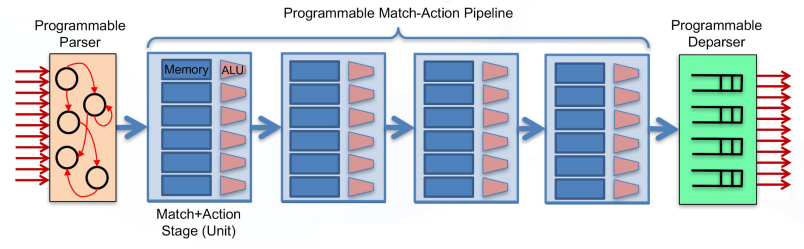
\includegraphics[width=1.0\columnwidth]{Figures/MatchAction.png}
		\rule{35em}{0.5pt}
	\caption[Match Action Pipeline]{Generic Data Programmable Switch Architecture}
	\label{fig:Match Action}
\end{figure}

\subsection{Constraints in data plane programmable switches}
In order to maintain processing at line-rate with no slow down, certain constraints need to be followed which impose a limit on the packet processing flexibility. Some of these are:
\begin{itemize}
  \item No looping constructs in P4 (language used to program switches)
  \item no floating point computations
  \item no exact multiply/divides (only approximated by bit-shifts)
  \item only one read-modify-write per stage to maintain processing at line rate
\end{itemize}
Even so, data plane programmability has found a number of applications in recent years including Network Monitoring and Debugging (the subject matter of this thesis), time synchronization, detection of elephant or heavy hitter flows, and In-network Computing.
\subsection{The P4 Programming Language}

P4 (\textit{Programming Protocol Independent Packet Processors}) is a programming language developed specifically for programming data plane switches. The language is maintained by the P4 Language Consortium and is widely used for data plane programmability today. It provides constructs for specifying deterministic parsers for header parsing, action constructs for specifying steps to be taken in case of a match, and also steps to be taken in packet reassembly.
%----------------------------------------------------------------------------------------

% \section{Getting Started with this Template}

% If you are familiar with \LaTeX{}, then you can familiarise yourself with the contents of the Zip file and the directory structure and then place your own information into the `\texttt{Thesis.cls}' file. Section \ref{FillingFile} on page \pageref{FillingFile} tells you how to do this. Make sure you read section \ref{ThesisConventions} about thesis conventions to get the most out of this template and then get started with the `\texttt{Thesis.tex}' file straightaway.

% If you are new to \LaTeX{} it is recommended that you carry on reading through the rest of the information in this document.

% \subsection{About this Template}

% This \LaTeX{} Thesis Template is originally based and created around a \LaTeX{} style file created by Steve R.\ Gunn from the University of Southampton (UK), department of Electronics and Computer Science. You can find his original thesis style file at his site, here:\\
% \href{http://www.ecs.soton.ac.uk/~srg/softwaretools/document/templates/}{\texttt{http://www.ecs.soton.ac.uk/$\sim$srg/softwaretools/document/templates/}}

% My thesis originally used the `\texttt{ecsthesis.cls}' from his list of styles. However, I knew \LaTeX{} could still format better. To get the look I wanted, I modified his style and also created a skeleton framework and folder structure to place the thesis files in.

% This Thesis Template consists of that modified style, the framework and the folder structure. All the work that has gone into the preparation and groundwork means that all you have to bother about is the writing.

% Before you begin using this template you should ensure that its style complies with the thesis style guidelines imposed by your institution. In most cases this template style and layout will be suitable. If it is not, it may only require a small change to bring the template in line with your institution's recommendations.

% %----------------------------------------------------------------------------------------

% \section{What this Template Includes}

% \subsection{Folders}

% This template comes as a single Zip file that expands out to many files and folders. The folder names are mostly self-explanatory:

% \textbf{Appendices} -- this is the folder where you put the appendices. Each appendix should go into its own separate `\texttt{.tex}' file. A template is included in the directory.

% \textbf{Chapters} -- this is the folder where you put the thesis chapters. A thesis usually has about seven chapters, though there is no hard rule on this. Each chapter should go in its own separate `\texttt{.tex}' file and they usually are split as:
% \begin{itemize}
% \item Chapter 1: Introduction to the thesis topic
% \item Chapter 2: Background information and theory
% \item Chapter 3: (Laboratory) experimental setup
% \item Chapter 4: Details of experiment 1
% \item Chapter 5: Details of experiment 2
% \item Chapter 6: Discussion of the experimental results
% \item Chapter 7: Conclusion and future directions
% \end{itemize}
% This chapter layout is specialised for the experimental sciences.

% \textbf{Figures} -- this folder contains all figures for the thesis. These are the final images that will go into the thesis document.

% \textbf{Primitives} -- this is the folder that contains scraps, particularly because one final image in the `Figures' folder may be made from many separate images and photos, these source images go here. This keeps the intermediate files separate from the final thesis figures.

% \subsection{Files}

% Included are also several files, most of them are plain text and you can see their contents in a text editor. Luckily, many of them are auxiliary files created by \LaTeX{} or BibTeX and which you don't need to bother about:

% \textbf{Bibliography.bib} -- this is an important file that contains all the bibliographic information and references that you will be citing in the thesis for use with BibTeX. You can write it manually, but there are reference manager programs available that will create and manage it for you. Bibliographies in \LaTeX{} are a large subject and you may need to read about BibTeX before starting with this.

% \textbf{Thesis.cls} -- this is an important file. It is the style file that tells \LaTeX{} how to format the thesis. You will also need to open this file in a text editor and fill in your own information (such as name, department, institution). Luckily, this is not too difficult and is explained in section \ref{FillingFile} on page \pageref{FillingFile}.

% \textbf{Thesis.pdf} -- this is your beautifully typeset thesis (in the PDF file format) created by \LaTeX{}.

% \textbf{Thesis.tex} -- this is an important file. This is the file that you tell \LaTeX{} to compile to produce your thesis as a PDF file. It contains the framework and constructs that tell \LaTeX{} how to layout the thesis. It is heavily commented so you can read exactly what each line of code does and why it is there. After you put your own information into the `\texttt{Thesis.cls}' file, go to this file and begin filling it in -- you have now started your thesis!

% \textbf{vector.sty} -- this is a \LaTeX{} package, it tells \LaTeX{} how to typeset mathematical vectors. Using this package is very easy and you can read the documentation on the site (you just need to look at the `\texttt{vector.pdf}' file):\\
% \href{http://www.ctan.org/tex-archive/macros/latex/contrib/vector/}{\texttt{http://www.ctan.org/tex-archive/macros/latex/contrib/vector/}}

% \textbf{lstpatch.sty} -- this is a \LaTeX{} package required by this LaTeX template and is included as not all \TeX{} distributions have it installed by default. You do not need to modify this file.

% Files that are \emph{not} included, but are created by \LaTeX{} as auxiliary files include:

% \textbf{Thesis.aux} -- this is an auxiliary file generated by \LaTeX{}, if it is deleted \LaTeX{} simply regenerates it when you run the main `\texttt{.tex}' file.

% \textbf{Thesis.bbl} -- this is an auxiliary file generated by BibTeX, if it is deleted, BibTeX simply regenerates it when you run the main tex file. Whereas the `\texttt{.bib}' file contains all the references you have, this `\texttt{.bbl}' file contains the references you have actually cited in the thesis and is used to build the bibliography section of the thesis.

% \textbf{Thesis.blg} -- this is an auxiliary file generated by BibTeX, if it is deleted BibTeX simply regenerates it when you run the main `\texttt{.tex}' file.

% \textbf{Thesis.lof} -- this is an auxiliary file generated by \LaTeX{}, if it is deleted \LaTeX{} simply regenerates it when you run the main `\texttt{.tex}' file. It tells \LaTeX{} how to build the `List of Figures' section.

% \textbf{Thesis.log} -- this is an auxiliary file generated by \LaTeX{}, if it is deleted \LaTeX{} simply regenerates it when you run the main `\texttt{.tex}' file. It contains messages from \LaTeX{}, if you receive errors and warnings from \LaTeX{}, they will be in this `\texttt{.log}' file.

% \textbf{Thesis.lot} -- this is an auxiliary file generated by \LaTeX{}, if it is deleted \LaTeX{} simply regenerates it when you run the main `\texttt{.tex}' file. It tells \LaTeX{} how to build the `List of Tables' section.

% \textbf{Thesis.out} -- this is an auxiliary file generated by \LaTeX{}, if it is deleted \LaTeX{} simply regenerates it when you run the main `\texttt{.tex}' file.


% So from this long list, only the files with the `\texttt{.sty}', `\texttt{.bib}', `\texttt{.cls}' and `\texttt{.tex}' extensions are the most important ones. The other auxiliary files can be ignored or deleted as \LaTeX{} and BibTeX will regenerate them.

% %----------------------------------------------------------------------------------------

% \section{Filling in the `\texttt{Thesis.cls}' File}\label{FillingFile}

% You will need to personalise the thesis template and make it your own by filling in your own information. This is done by editing the `\texttt{Thesis.cls}' file in a text editor.

% Open the file and scroll down, past all the `$\backslash$\texttt{newcommand}\ldots' items until you see the entries for `\texttt{University Name}', `\texttt{Department Name}', etc\ldots.

% Fill out the information about your group and institution and ensure you keep to block capitals where it asks you to. You can also insert web links, if you do, make sure you use the full URL, including the `\texttt{http://}' for this.

% The last item you should need to fill in is the Faculty Name (in block capitals). When you have done this, save the file and recompile `\texttt{Thesis.tex}'. All the information you filled in should now be in the PDF, complete with web links. You can now begin your thesis proper!

% %----------------------------------------------------------------------------------------

% \section{The `\texttt{Thesis.tex}' File Explained}

% The \texttt{Thesis.tex} file contains the structure of the thesis. There are plenty of written comments that explain what pages, sections and formatting the \LaTeX{} code is creating. Initially there seems to be a lot of \LaTeX{} code, but this is all formatting, and it has all been taken care of so you don't have to do it.

% Begin by checking that your information on the title page is correct. For the thesis declaration, your institution may insist on something different than the text given. If this is the case, just replace what you see with what is required.

% Then comes a page which contains a funny quote. You can put your own, or quote your favourite scientist, author, person, etc\ldots Make sure to put the name of the person who you took the quote from.

% Next comes the acknowledgements. On this page, write about all the people who you wish to thank (not forgetting parents, partners and your advisor/supervisor).

% The contents pages, list of figures and tables are all taken care of for you and do not need to be manually created or edited. The next set of pages are optional and can be deleted since they are for a more technical thesis: insert a list of abbreviations you have used in the thesis, then a list of the physical constants and numbers you refer to and finally, a list of mathematical symbols used in any formulae. Making the effort to fill these tables means the reader has a one-stop place to refer to instead of searching the internet and references to try and find out what you meant by certain abbreviations or symbols.

% The list of symbols is split into the Roman and Greek alphabets. Whereas the abbreviations and symbols ought to be listed in alphabetical order (and this is \emph{not} done automatically for you) the list of physical constants should be grouped into similar themes.

% The next page contains a one line dedication. Who will you dedicate your thesis to?

% Finally, there is the section where the chapters are included. Uncomment the lines (delete the `\texttt{\%}' character) as you write the chapters. Each chapter should be written in its own file and put into the `Chapters' folder and named `\texttt{Chapter1}', `\texttt{Chapter2}, etc\ldots Similarly for the appendices, uncomment the lines as you need them. Each appendix should go into its own file and placed in the `Appendices' folder.

% After the preamble, chapters and appendices finally comes the bibliography. The bibliography style (called `\texttt{unsrtnat}') is used for the bibliography and is a fully featured style that will even include links to where the referenced paper can be found online. Do not under estimate how grateful you reader will be to find that a reference to a paper is just a click away. Of course, this relies on you putting the URL information into the BibTeX file in the first place.

% %----------------------------------------------------------------------------------------

% \section{Thesis Features and Conventions}\label{ThesisConventions}

% To get the best out of this template, there are a few conventions that you may want to follow.

% One of the most important (and most difficult) things to keep track of in such a long document as a thesis is consistency. Using certain conventions and ways of doing things (such as using a Todo list) makes the job easier. Of course, all of these are optional and you can adopt your own method.

% \subsection{Printing Format}

% This thesis template is designed for single sided printing as most theses are printed and bound this way. This means that the left margin is always wider than the right (for binding). Four out of five people will now judge the margins by eye and think, ``I never 
% noticed that before.''.

% The headers for the pages contain the page number on the right side (so it is easy to flick through to the page you want) and the chapter name on the left side.

% The text is set to 11 point and a line spacing of 1.3. Generally, it is much more readable to have a smaller text size and wider gap between the lines than it is to have a larger text size and smaller gap. Again, you can tune the text size and spacing should you want or need to. The text size can be set in the options for the `$\backslash$\texttt{documentclass}' command at the top of the `\texttt{Thesis.tex}' file and the spacing can be changed by setting a different value in the `$\backslash$\texttt{setstretch}' commands (scattered throughout the `\texttt{Thesis.tex}' file).

% \subsection{Using US Letter Paper}

% The paper size used in the template is A4, which is a common -- if not standard -- size in Europe. If you are using this thesis template elsewhere and particularly in the United States, then you may have to change the A4 paper size to the US Letter size. Unfortunately, this is not as simple as replacing instances of `\texttt{a4paper}' with `\texttt{letterpaper}'.

% This is because the final PDF file is created directly from the \LaTeX{} source using a program called `\texttt{pdfTeX}' and in certain conditions, paper size commands are ignored and all documents are created with the paper size set to the size stated in the configuration file for pdfTeX (called `\texttt{pdftex.cfg}').

% What needs to be done is to change the paper size in the configuration file for \texttt{pdfTeX} to reflect the letter size. There is an excellent tutorial on how to do this here: \\
% \href{http://www.physics.wm.edu/~norman/latexhints/pdf_papersize.html}{\texttt{http://www.physics.wm.edu/$\sim$norman/latexhints/pdf\_papersize.html}}

% It may be sufficient just to replace the dimensions of the A4 paper size with the US Letter size in the \texttt{pdftex.cfg} file. Due to the differences in the paper size, the resulting margins may be different to what you like or require (as it is common for Institutions to dictate certain margin sizes). If this is the case, then the margin sizes can be tweaked by opening up the \texttt{Thesis.cls} file and searching for the line beginning with, `$\backslash$\texttt{setmarginsrb}' (not very far down from the top), there you will see the margins specified. Simply change those values to what you need (or what looks good) and save. Now your document should be set up for US Letter paper size with suitable margins.

% \subsection{References}

% The `\texttt{natbib}' package is used to format the bibliography and inserts references such as this one \cite{cmu-malware}. The options used in the `\texttt{Thesis.tex}' file mean that the references are listed in numerical order as they appear in the text. Multiple references are rearranged in numerical order (e.g. \cite{kendall2007practical}). This is done automatically for you. To see how you use references, have a look at the `\texttt{Chapter1.tex}' source file. Many reference managers allow you to simply drag the reference into the document as you type.

% Scientific references should come \emph{before} the punctuation mark if there is one (such as a comma or period). The same goes for footnotes\footnote{Such as this footnote, here down at the bottom of the page.}. You can change this but the most important thing is to keep the convention consistent throughout the thesis. Footnotes themselves should be full, descriptive sentences (beginning with a capital letter and ending with a full stop).

% To see how \LaTeX{} typesets the bibliography, have a look at the very end of this document (or just click on the reference number links).

%----------------------------------------------------------------------------------------
